% Overview : capabilities.tex
% Explain what capability additions have resulted from benchmarking

\begin{frame}
  \frametitle{Cyclus Modular Architecture and Open Development}
  The combination of modular encapsulation within the software
  architecture and an open development paradigm allows for simulation
  at multiple levels of simulation detail.
\end{frame}

% \begin{frame}[ctb!]
%   \frametitle{Encapsulation}
%   \begin{figure}[htbp!]
%     \begin{center}
%       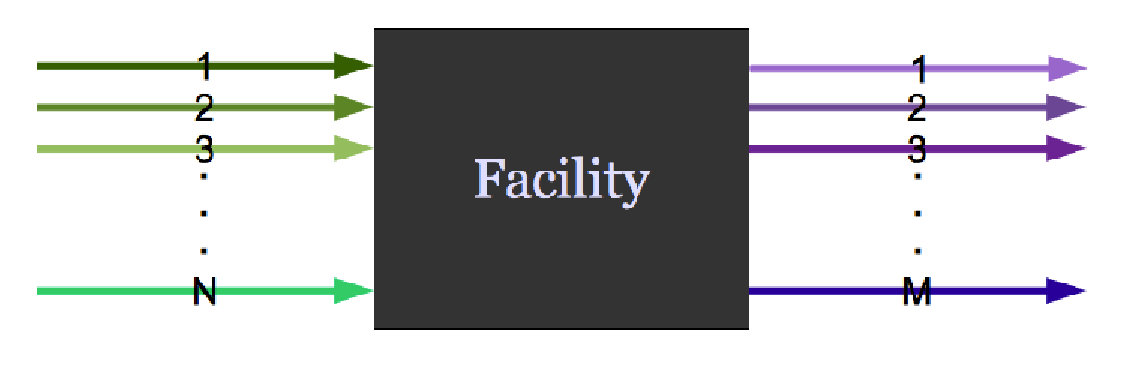
\includegraphics[height=5cm]{facility.eps}
%     \end{center}
%     \caption{ Regions, Institutions, Facilities, and Markets are all
%     black boxes.} 
%     \label{fig:sinkfacility}
%   \end{figure}
% \end{frame}

% \begin{frame}[ctb!]
%   \frametitle{Module Interfaces}
%   \begin{figure}[htbp!]
%     \begin{center}
%       \includegraphics[height=5cm]{interfaces.eps}
%     \caption{Well defined model interfaces facilitate model 
%     interchange. The user may choose the model at their desired level  
%     of detail.}
%     \label{fig:interfaces}
%     \end{center}
%   \end{figure}
% \end{frame}

% \begin{frame}[ctb!]
%   \frametitle{Facilities Are Black Boxes}
%   \begin{figure}[htbp!]
%     \begin{center}
%       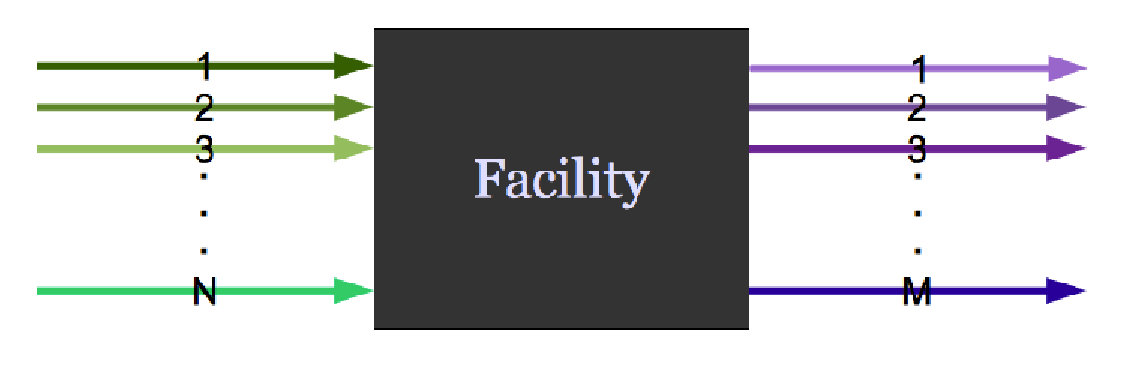
\includegraphics[height=5cm]{facility.eps}
%     \end{center}
%     \caption{ Each facility in the simulation makes requests and offers 
%     to fill its stocks and empty its inventory respectively.  }
%     \label{fig:facility}
%   \end{figure}
% \end{frame}

% \begin{frame}[ctb!]
%   \frametitle{Facilities Are Black Boxes}
%   \begin{figure}[htbp!]
%     \begin{center}
%       \includegraphics[height=5cm]{sourcefacility.eps}
%     \end{center}
%     \caption{ A facility might only make offers.} 
%     \label{fig:sourcefacility}
%   \end{figure}
% \end{frame}

% \begin{frame}[ctb!]
%   \frametitle{Facilities Are Black Boxes}
%   \begin{figure}[htbp!]
%     \begin{center}
%       \includegraphics[height=5cm]{sinkfacility.eps}
%     \end{center}
%     \caption{ A facility might only make requests.} 
%     \label{fig:sinkfacility}
%   \end{figure}
% \end{frame}
